\documentclass{article}

\usepackage{amsmath}
\usepackage{graphicx}
\graphicspath{/home/mike/Desktop/Powers and Roots}
\usepackage{tikz}
\usepackage{cancel}
\usepackage{setspace}
\usepackage[fontsize=16pt]{fontsize}

\author{Mike \& Paula McLennan}
\date{}
\title{Powers and Roots\\
\vspace{28pt}
\begin{normalsize}Applied Scholastics, Ferndale WA \end{normalsize}}

\begin{document}

\maketitle
\pagebreak
\tableofcontents
\pagebreak

\begin{spacing}{1.25}

\section{Powers}
Power means size and strength. When a number is multiplied by itself over and over, you raise it to a higher power. It gets bigger and it is called a power of that number.

\vspace{28pt}
An example is the powers of 3:

The first power of 3 is just 3.

The second power of 3 is $3 \times 3 = 9.$

The third power of 3 is $3 \times 3 \times 3 = 27.$

\vspace{28pt}
And so on. You get the idea?

\pagebreak

\subsection*{Writing Powers}

Root means the base of something or where things grow from, like the root of a tree.

\begin{center}
$3 \times 3 \times 3$\\
$3 \times 3$\\
$3$
\end{center}

The number being multiplied is called the root, and the number of times it is multiplied by itself is called the power.\\

You write the power as a small raised number to the right of the root.

\begin{center}
$\text{root}\rightarrow$
{\fontsize{30}{34}\selectfont 3}
$\textsuperscript{{\fontsize{15}{20}\selectfont 5} $\longleftarrow$}\textsuperscript{\normalsize{\text{power}}}$
\normalsize
\end{center}

Its written that way because its shorter, rather than having to write out in full that number of multiplications, so $3^5 \text{ means }3 \times 3 \times 3 \times 3 \times 3.$\\

Sometimes, we use the {\fontsize{30}{30}\selectfont {\string^}} symbol when writing on a computer instead of the small raised number, so $3^5$ would be written as 3{\fontsize{30}{34}\selectfont {\string^}}5.

\pagebreak

\subsection*{Reading Powers}

When you are reading a number that is written with a power, such as $3^5$, there are a few different ways of saying it.\\

You can call it the fifth power of 3.\\

You can say 3 raised to the fifth power.\\

You can say 3 to the fifth power.\\

Or you can just say 3 to the fifth.

\pagebreak

\subsection*{Index}

Index means a pointer, like the index of a book points to where you can find things in it. The power of a number can also be called the index because it points to what power the number is being raised to.

\begin{center}
$\text{root}\rightarrow$
{\fontsize{30}{34}\selectfont 3}
$\textsuperscript{{\fontsize{15}{20}\selectfont 5} $\longleftarrow$}\textsuperscript{\normalsize{\text{index}}}$
\normalsize
\end{center}

If you are talking about more than one index, you don’t say indexes. The 2 and the 3 in $5^2+6^3$ are called indices, and you say it as \textit{indisees.}

\subsubsection*{Exponent}

Exponent means a person or thing which explains or makes clear. American maths books use the word exponent instead of index or power.

\begin{center}
$\text{root}\rightarrow$
{\fontsize{30}{34}\selectfont 3}
$\textsuperscript{{\fontsize{15}{20}\selectfont 5} $\longleftarrow$}\textsuperscript{\normalsize{\text{exponent}}}$
\normalsize
\end{center}

\pagebreak

\subsection*{Squares}

A square has sides of equal length. Area means the size of a flat surface. To find the area of a square you multiply the length of the two sides.\\

\begin{figure}
  \centering
  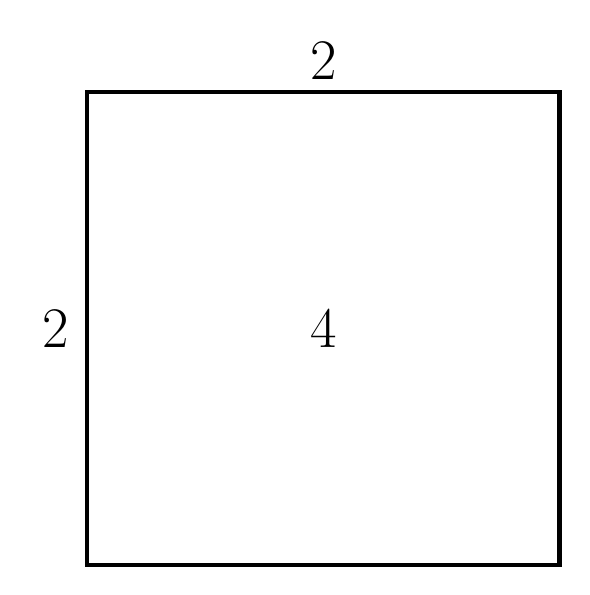
\begin{tikzpicture}
    \draw [ultra thick](0,0) rectangle (6,6);
%    \fill[lightgray] (0,0) rectangle (6,6);
    \node at (3,3) {\fontsize{20}{24}\selectfont 4};
    \node at (-0.4,3) {\fontsize{20}{24}\selectfont 2};
    \node at (3,6.4) {\fontsize{20}{24}\selectfont 2};
  \end{tikzpicture}
  \quad
  \begin{minipage}{5cm}
    \[
    \text{Area} = 2 \times 2 = 2^2 = 4
    \]
  \end{minipage}
\end{figure}

That's why multiplying a number by itself is called squaring the number.\\

 You wouldn't call it 2 to the second power or anything. You would say the square of 2 is 4 or that 2 squared is 4.

\pagebreak

\subsection*{Cubes}

Volume means the size of something and how much space it takes up, not just a flat area.
A cube has 3 sides all of the same length.
That's why a number that has been multiplied by itself 3 times is called the cube of that number.

To find the volume of a cube, how big it is, you multiply the length of its side by itself 3 times. You would say the cube of 2 is 8, or 2 cubed is 8.

\vspace{28pt}

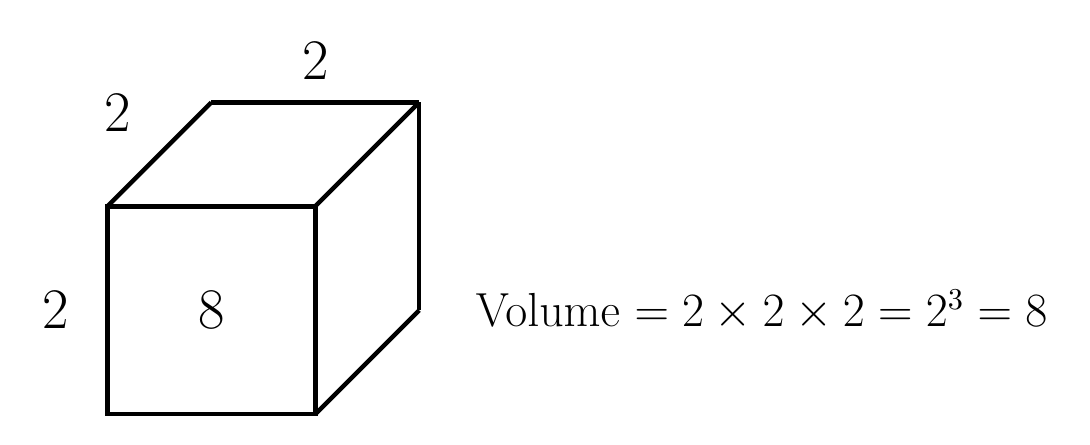
\begin{tikzpicture}[scale=0.66]
% Draw square with thick lines
\draw[ultra thick] (0, 0) rectangle (4, 4);
%\draw[ultra thick, fill=lightgray] (0, 0) rectangle (4, 4);
% Place "8" in the center with larger font size
\node at (2, 2) {\fontsize{20}{24}\selectfont 8};
% Place "2" to the left of the square with larger font size
\node at (-1, 2) {\fontsize{20}{24}\selectfont 2};
% Draw line from top left of square with thick line
\draw[ultra thick] (0, 4) -- (2, 6);
% Place "2" above the line with larger font size
\node at (0.2, 5.8) {\fontsize{20}{24}\selectfont 2};
% Draw line from top right of square with thick line
\draw[ultra thick] (4, 4) -- (6, 6);
% Connect the two lines with a horizontal line with thick line
\draw[ultra thick] (2, 6) -- (6, 6);
% Place "2" above the line with larger font size
\node at (4, 6.8) {\fontsize{20}{24}\selectfont 2};
% Shade the area with gray
%\fill[gray] (0, 4) -- (2, 6) -- (6, 6) -- (4, 4) -- cycle;
% Draw line from bottom right of square with thick line
\draw[ultra thick] (4, 0) -- (6, 2);
% Draw vertical line from the end of the previous line with thick line
\draw[ultra thick] (6, 2) -- (6, 6);
% Shade the area with lighter dark gray
%\fill[darkgray] (4, 0) -- (6, 2) -- (6, 6) -- (4,4) -- cycle;
% Write volume equation to the right with larger font size
\node[right] at (6.8, 2) {\fontsize{16}{19}\selectfont Volume $= 2 \times 2 \times 2 = 2^3 = 8$};
\end{tikzpicture}
\vspace{28pt}

\pagebreak

\section{Roots}

Sometimes you only have a power of a number and you want to find out the root that it started with. Just like you can find the power of a number, you can also find the root.

If you start with a root of 3 and multiply it by itself 3 times, you get $3 \times 3 \times 3 = 27$, the third power of 3. The number that you have to multiply by itself 3 times to get 27, is 3, so 3 is the third root of 27.\\

Say you are asked to find the fourth root 256. That means you need to find what number, when multiplied by itself 4 times, gives  256.
\begin{align*}
4^1 &= 4\\
4^2 &= 4 \times 4 = 16\\
4^3 &= 4 \times 4 \times 4 = 64\\
4^4 &= 4 \times 4 \times 4 \times 4 = 256
\end{align*}

As you can see, 256 is the fourth power of 4, so 4 is the fourth root of 256.

\pagebreak

Here is a list of the first powers of 3 :

\begin{center}
$3^1 = 3$
\end{center}
The first power of 3 is just 3, so the first root of 3 is also just 3.

\begin{center}
$3^2 = 3 \times 3 = 9$
\end{center}
3 raised to the second power is 9, so the second root of 9 is 3.

\begin{center}
$3^3 = 3 \times 3 \times 3 = 27$
\end{center}
3 raised to the third power is 27, so third root of 27 is 3.

\begin{center}
$3^4 = 3 \times 3 \times 3 \times 3 = 81$
\end{center}
3 raised to the fourth power is 81, so the fourth root of 81 is 3.

\begin{center}
$3^5 = 3 \times 3 \times 3 \times 3 \times 3 = 243$
\end{center}
3 raised to the fifth power is 243, so the fifth root of 243 is 3.

\pagebreak

\subsection*{The Root Symbol}

There’s a special symbol $\sqrt{}$ for finding roots called the root symbol.
You write the root symbol and then write the power with a line along the top of it, and the index to the left of the $\sqrt{}$ that indicates which root.\\

\begin{center}
index $\longrightarrow$ {\fontsize{40}{44}\selectfont {$\sqrt[5]{243} = 3$}}
$\longleftarrow$ root
\end{center}



\vspace{28pt}
$\sqrt[5]{243} = 3$ means that 3 is the number which multiplied by itself 5 times is 243. The 5\textsuperscript{th} root of 243 is 3.

\pagebreak

\subsection*{Square Roots}

The square of a number is the second power of the number, so the second root of a number is the square root.

For a square with an area of 4, the length of it’s sides must be 2. The square root of 4 is 2.

\begin{figure}
  \centering
  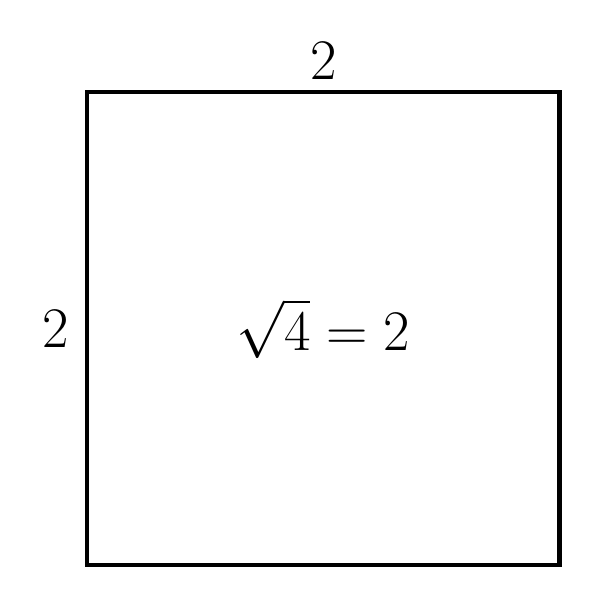
\begin{tikzpicture}
    \draw [ultra thick](0,0) rectangle (6,6);
%    \fill[lightgray] (0,0) rectangle (6,6);
    \node at (3,3) {\fontsize{20}{24}\selectfont $\sqrt{4} = 2$};
    \node at (-0.4,3) {\fontsize{20}{24}\selectfont 2};
    \node at (3,6.4) {\fontsize{20}{24}\selectfont 2};
  \end{tikzpicture}
  \quad
  \begin{minipage}{5cm}
    \[
    \text{Area} = 2 \times 2 = 2^2 = 4
    \]
  \end{minipage}
\end{figure}

If you see the $\sqrt{}$ symbol written without an index then its a square root.  $\sqrt[2]{16} = 4$ is just written as $\sqrt{16} = 4.$ It’s the most commonly used root so the 2 usually isn’t written.

\subsection*{Cube Roots}
\begin{align*}
27 &= 3^3\\
9 &= 3^2\\
3 &= 3^1
\end{align*}

The cube of a number is its third power, and its third root is called the cube root.

A cube with a volume of 27 must have sides with lengths of 3, so the cube root of 27 is 3.

\vspace{28pt}
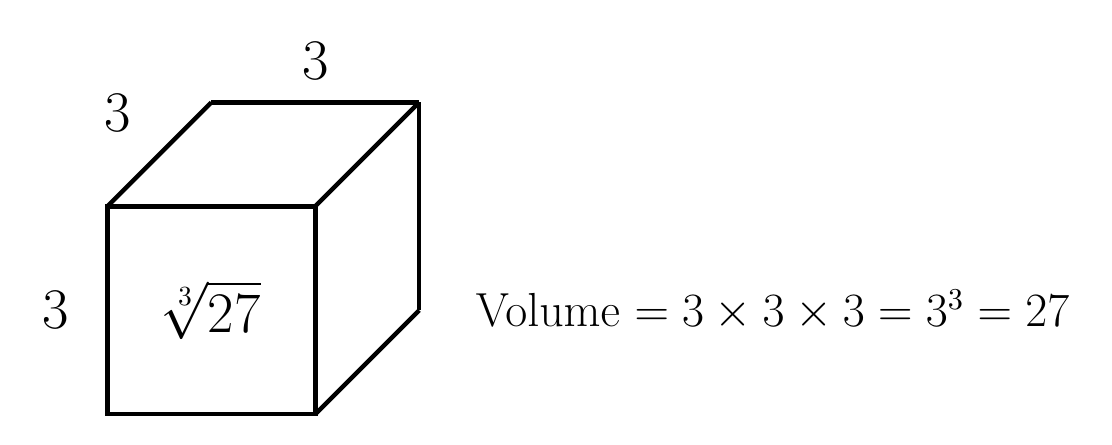
\begin{tikzpicture}[scale=0.66]
% Draw square with thick lines
%\draw[ultra thick, fill=lightgray] (0, 0) rectangle (4, 4);
\draw[ultra thick] (0, 0) rectangle (4, 4);
% Place "8" in the center with larger font size
\node at (2, 2) {\fontsize{20}{24}\selectfont $\sqrt[3]{27}$};
% Place "2" to the left of the square with larger font size
\node at (-1, 2) {\fontsize{20}{24}\selectfont 3};
% Draw line from top left of square with thick line
\draw[ultra thick] (0, 4) -- (2, 6);
% Place "2" above the line with larger font size
\node at (0.2, 5.8) {\fontsize{20}{24}\selectfont 3};
% Draw line from top right of square with thick line
\draw[ultra thick] (4, 4) -- (6, 6);
% Connect the two lines with a horizontal line with thick line
\draw[ultra thick] (2, 6) -- (6, 6);
% Place "2" above the line with larger font size
\node at (4, 6.8) {\fontsize{20}{24}\selectfont 3};
% Shade the area with gray
%\fill[gray] (0, 4) -- (2, 6) -- (6, 6) -- (4, 4) -- cycle;
% Draw line from bottom right of square with thick line
\draw[ultra thick] (4, 0) -- (6, 2);
% Draw vertical line from the end of the previous line with thick line
\draw[ultra thick] (6, 2) -- (6, 6);
% Shade the area with lighter dark gray
%\fill[darkgray] (4, 0) -- (6, 2) -- (6, 6) -- (4,4) -- cycle;
% Write volume equation to the right with larger font size
\node[right] at (6.8, 2) {\fontsize{16}{19}\selectfont Volume $= 3 \times 3 \times 3 = 3^3 = 27$};
\end{tikzpicture}

\vspace{28pt}
You would write $\sqrt[3]{27} = 3$.

\pagebreak

\section*{Practice}

\begin{enumerate}
\item What is 2 to the power of 4?\\
\item What is the square root of 64?\\
\item What is the cube root of 27?\\
\item What is 5 to the power of 3?\\
\item What is the fourth power of 2?\\
\item What is 3 raised to the fourth power?\\
\item What is the fourth root of 81?\\
\item What is 4 cubed?
\end{enumerate}

\pagebreak

\subsection*{Answers}

\begin{enumerate}
\item $2^4 = 2 \times 2 \times 2 \times 2 = 16$\\
\item $\sqrt{64} = 8$\\
\item $\sqrt[3]{27} = 3$\\
\item $5^3 = 5 \times 5 \times 5 = 125$\\
\item $2^4 = 2 \times 2 \times 2 \times 2 = 16$\\
\item $3^4 = 3 \times 3 \times 3 \times 3 = 81$\\
\item $3^4 = 81\ \text{so}\ \sqrt[4]{81} = 3$\\
\item $4^3 = 4 \times 4 \times 4 = 64$
\end{enumerate}

\pagebreak

\doublespacing

\begin{center}

Enquiries

\textbf{Applied Scholastics Ferndale}

Principal: Paula McLennan

mobile phone: 0431 683 306

email address: apsferndale@gmail.com

website: apsferndale.webs.com
\end{center}

\end{spacing}
\end{document}
